\section{Numerical experiments}

In order to test that the model makes sense from a physical
perspective, simulation experiments have been conducted. Expertise
from FLIR has provided metrics against which outputs from the model
has been benchmarked, along with suggestions for electronic design
experiments. Below the resulting experiments are presented along with
benchmarks if applicable.


\subsection{Solution with noisy model}
For the parameter $\sigma$, we set as a baseline
\begin{align}
\sigma = \sqrt{4KT_sR(T_s)}
\end{align}
where  $K$ is the Boltzmann constant. This value is of order $1e^{-7}$
and is possible to motivate from a physical perspective. A detailed
explanation can be found in~\cite{WOOD199743}.

We will however amplify or diminish $\sigma$ depending on our needs
with a constant $d$. Thus we will use
\begin{align}
\sigma = d \sqrt{4KT_sR(T_s)}
\end{align}

Plots from running the temperature simulation and succeeding
integrator with the noisy scheme outlined in
Equation~\eqref{eq:heat_balance_equation_noise_discr} are shown
in Figure~\ref{fig:noisysol}. We see that the difference from the
deterministic solution is marginal, even with amplified noise.

\begin{figure}
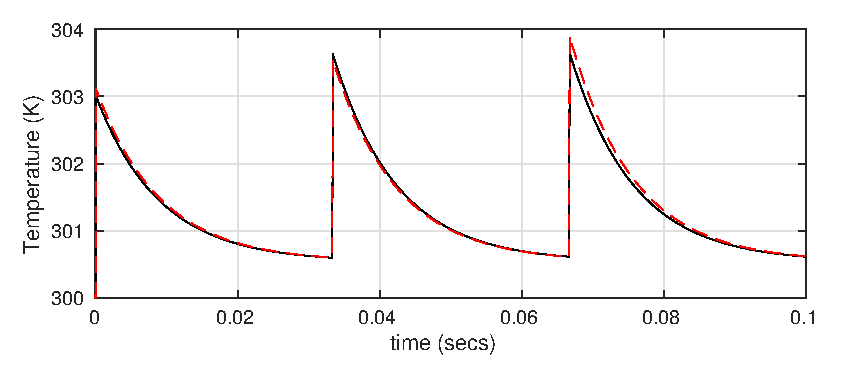
\includegraphics[scale=0.9]{gfx/sol_several_pulses_noise.eps}
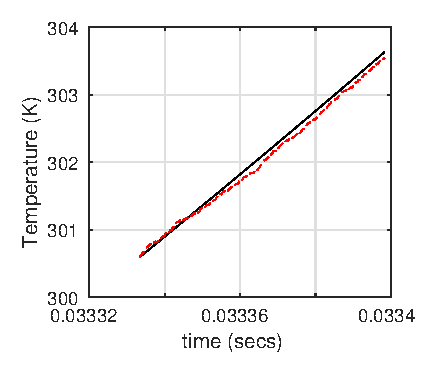
\includegraphics[scale=0.9]{gfx/sol_int_time_noise.eps}
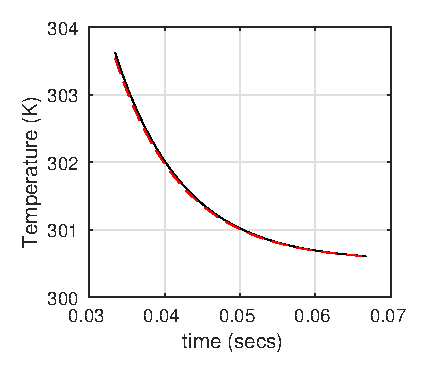
\includegraphics[scale=0.9]{gfx/sol_cooling_noise.eps}
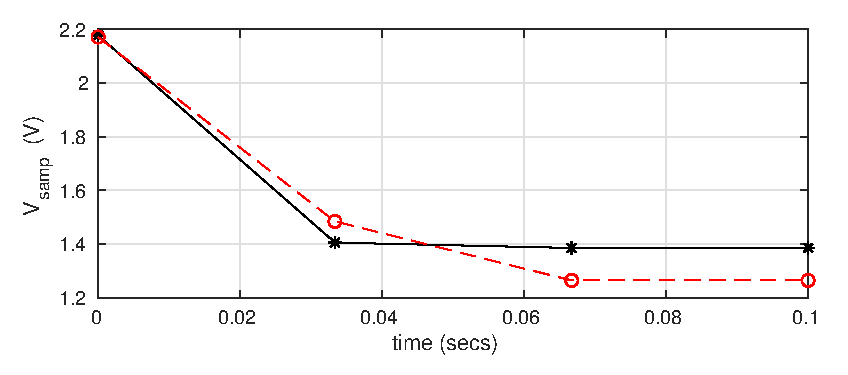
\includegraphics[scale=0.9]{gfx/Vout_several_pulses_noise.eps}
\caption{Temperature and output signal development over time for
  $d=100$. Red: Noisy solution, Black: Deterministic solution}
\label{fig:noisysol}
\end{figure}


\subsection{Investigating model accuracy as function of $\sigma$}
The model accuracy can be measured with the Noise Equivalent Temperature Difference (NETD), which has form
\begin{align}
\mbox{NETD} = \frac{std(V(T, \sigma))}{V(T+1,0)-V(T,0)}
\end{align}
It compares the standard deviation of the noisy output signal at temperature $T$ with the difference in a deterministic signal when heating the observed object
from $T$ to $T+1$. In other words, a large NETD indicates that the noise in the output is too large to detect a change of 1 degree in the observed object.
Figure~\ref{fig:NETD_over_sigma} depicts NETD over $\sigma$ at $T=300$. At this temperature, FLIR has estimated NETD to 20 mK.
This knowledge lets us solve $\sigma$ from the graph, resulting in a value of around $7e^{-6}$.
\begin{figure}[H]
 \begin{center}
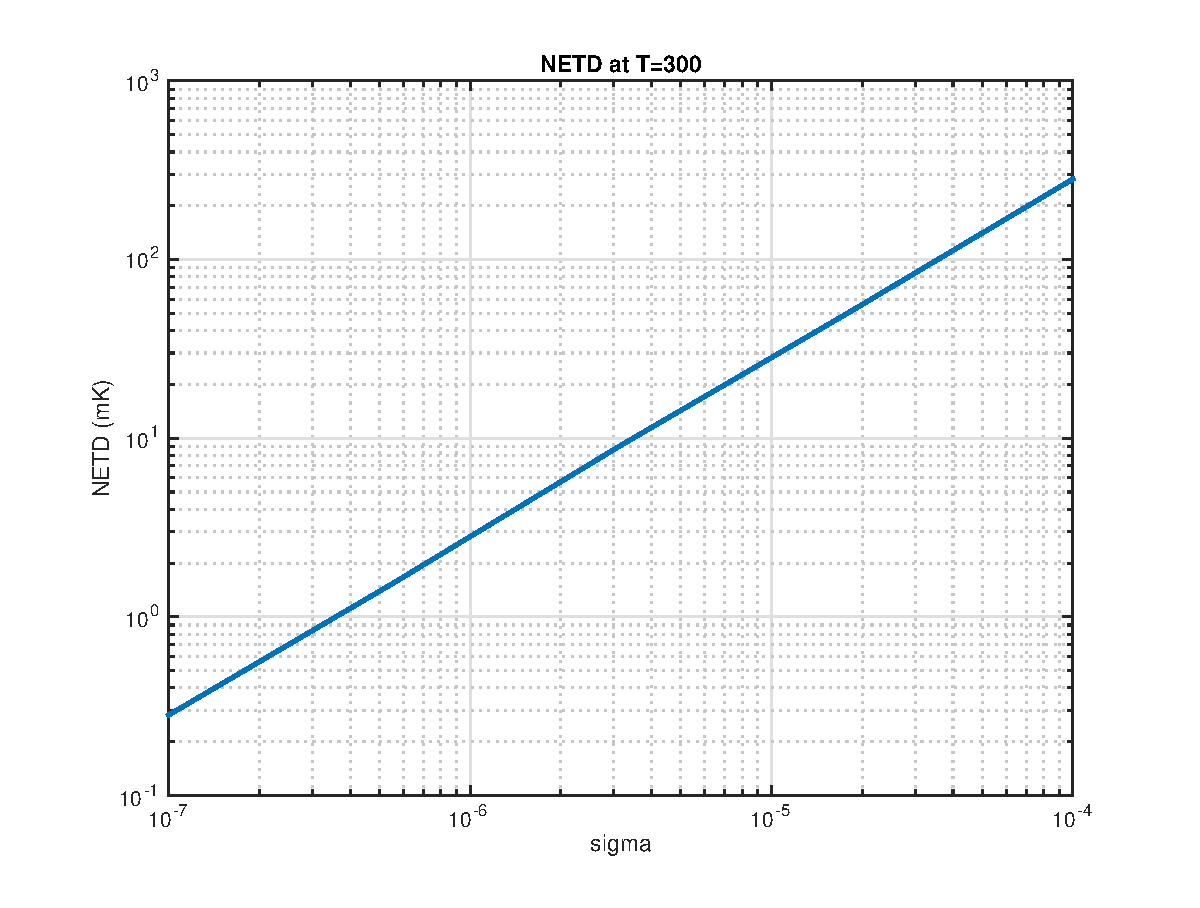
\includegraphics[scale=0.9]{gfx/NETD_as_function_of_sigma.eps}
  \caption{NETD as function of $\sigma$}
  \label{fig:NETD_over_sigma}
  \end{center}
\end{figure}

\subsection{Noise dependence on integration time}
Since measurements are collected only during integration time, a larger integration time on one hand acts to increase the measurement time-span and hence the
reliability of the measurement. On the other hand, a larger integration time infers more substantial heating of the thermistor, resulting in increased noise. It is therefore
of interest to investigate how the output noise depends on the integration time. In Figure~\ref{fig:std_over_time}, signal standard deviations for different frame rates
are plotted against simulations of different integration times. The curve grows approximately as $t^{3/2}$. FLIR has estimated the curve to grow approximately as $t^{1/2}$, indicating
our model is growing at too fast speed. This same peculiarity might explain that the plot of NETD over integration time is increasing, contrary to the experience at FLIR suggesting
a decreasing NETD-curve.
%\begin{figure}[H]
%    \centering
%    \subfloat[label 1]{{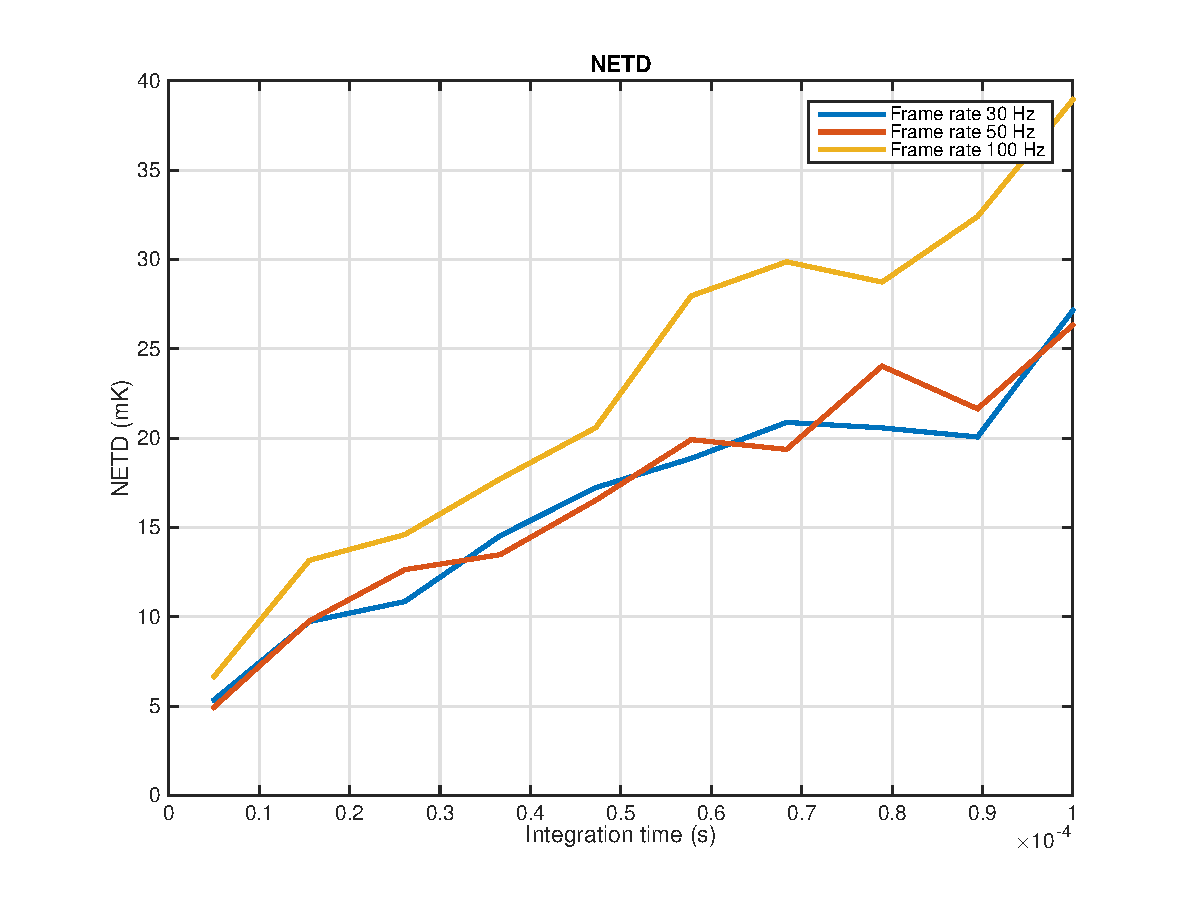
\includegraphics[width=5cm]{gfx/NETS_Function_of_Integration_Time.eps} }}
%    \qquad
%    \subfloat[label 2]{{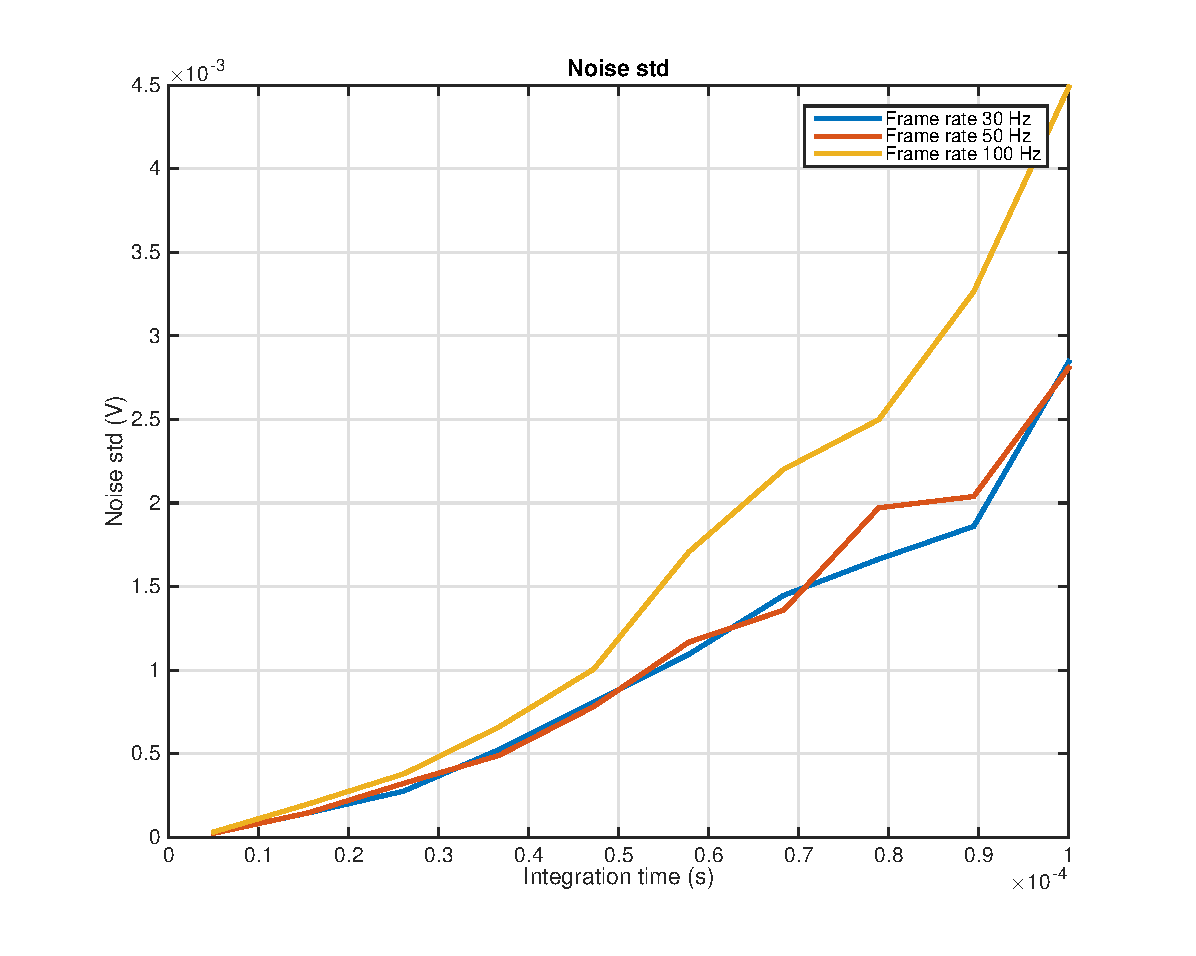
\includegraphics[width=5cm]{gfx/STD_Function_of_Integration_Time.eps} }}
%  \caption{Output standard deviation over integration time}
%  \label{fig:std_over_time}
%\end{figure}
\begin{figure}[H]
 \begin{center}
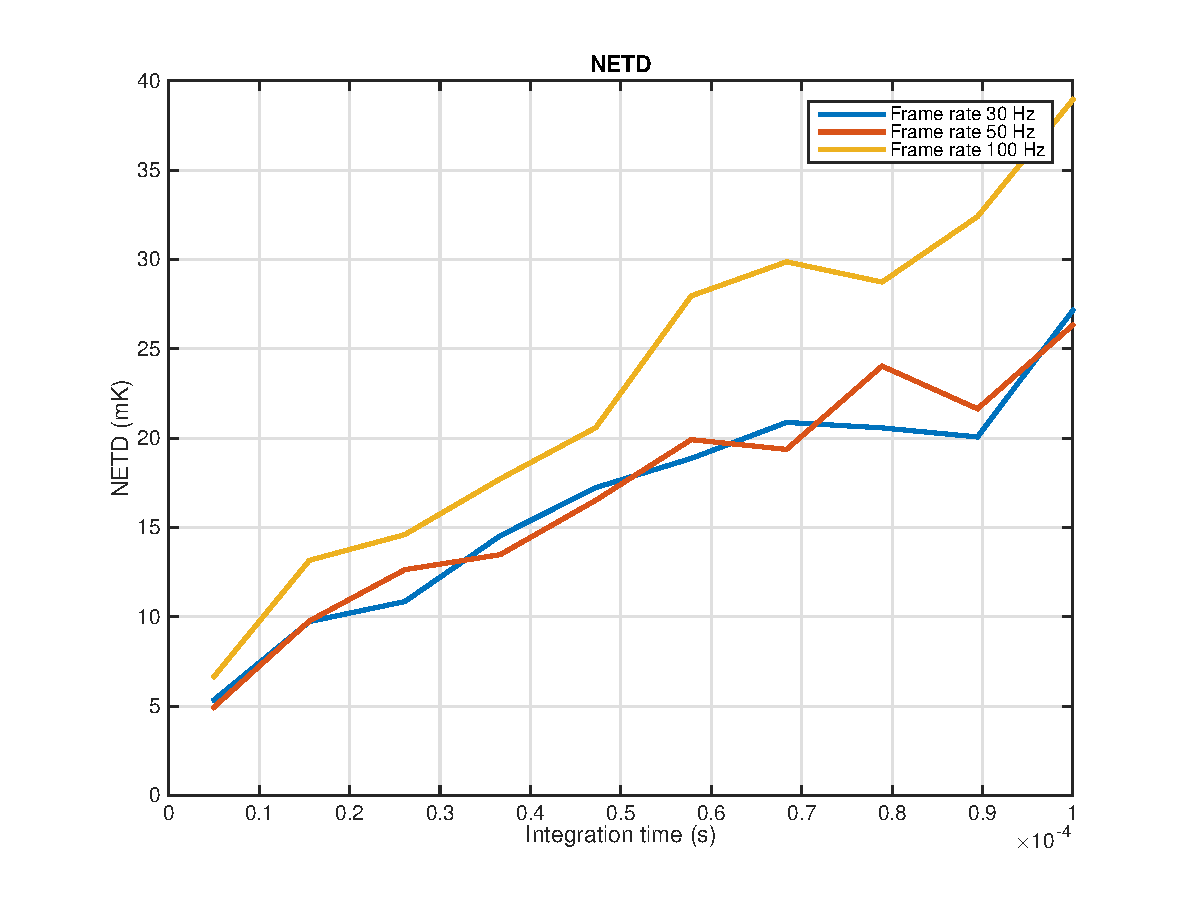
\includegraphics[scale=0.8]{gfx/NETS_Function_of_Integration_Time.eps}
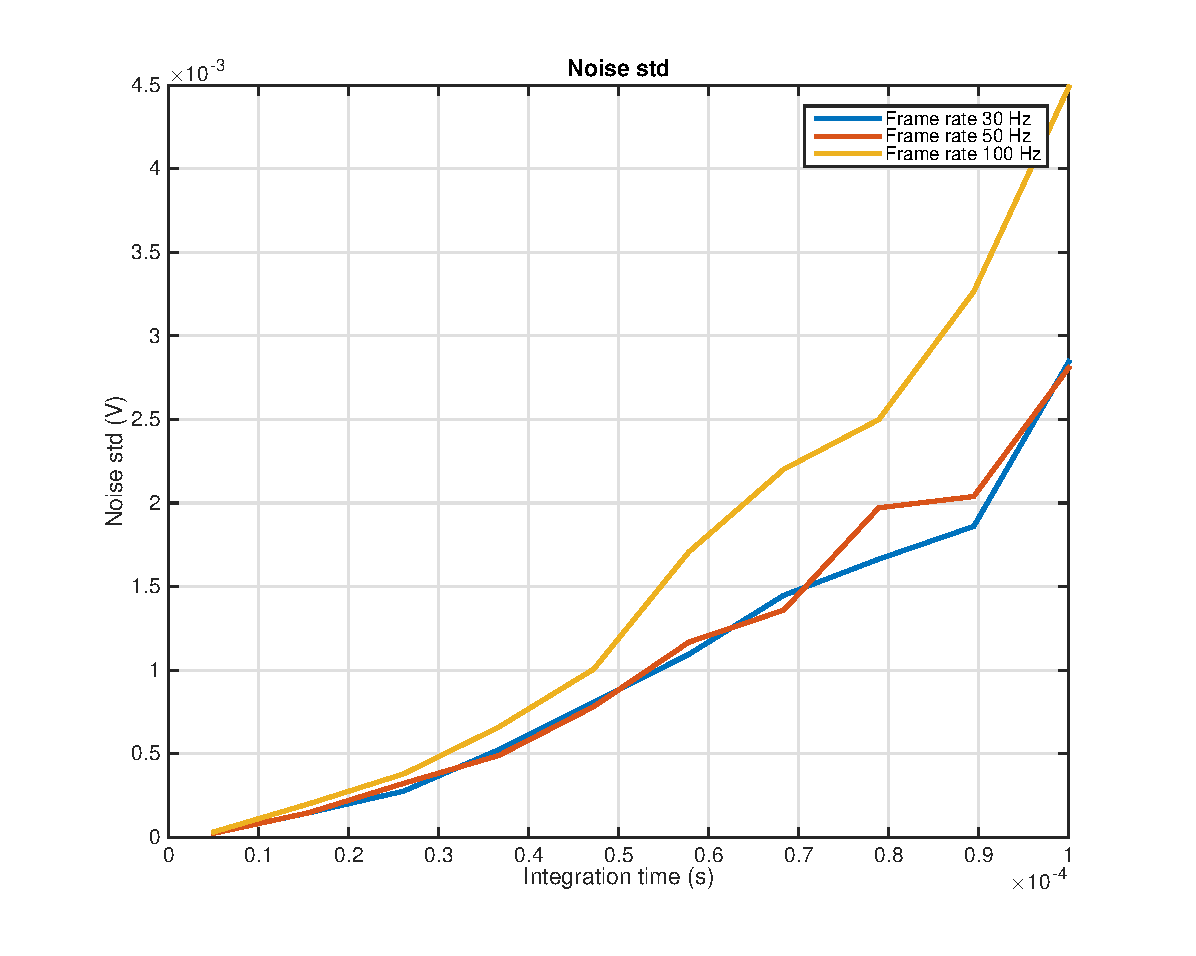
\includegraphics[scale=0.8]{gfx/STD_Function_of_Integration_Time.eps}
  \caption{Output standard deviation over integration time}
  \label{fig:std_over_time}
  \end{center}
\end{figure}


\subsection{Power spectrum of output signal}
Expertise from FLIR suggest that the power spectrum of the output signal is dependent on the frame-rate, and situated somewhere between the white and $1/f$ noise spectrum.
In order to test the accordance between this experience and the model, the power spectrum of the output signal for different frame-rates have been generated. The result can be seen in
Figure~\ref{fig:pspec}, together with a $1/f$ deterministic curve. Indeed, the output signal seems to shift from a white noise character to a $1/f$ character as frame-rates are altered.
\begin{figure}[H]
 \begin{center}
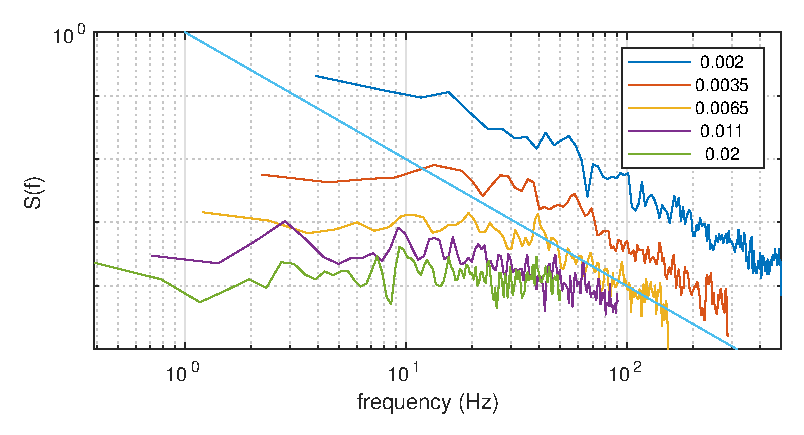
\includegraphics[scale=0.9]{gfx/pspec.eps}
  \caption{Power spectrum of output signal for different frame-rates $1/t_f$}
  \label{fig:pspec}
  \end{center}
\end{figure}

\subsection{Linearity of the output signal}
The linearity of the output signal as a function of incoming radiation effect is an assumption made during the calibration process at FLIR. The deviation of the signal from this assumption
require re-calibration of the camera at regular intervals. It is therefore of interest to investigate how this linearity is affected by factors possible to influence by design. For example, FLIR suggest that the design of the bias voltage curve during integration time might be important to achieve a higher degree of linearity in the output signal. In Figure~\ref{fig:out_vs_inrad}, output signals $V_{samp}$ over incoming effect $P_{t}$ are plotted for different designs of bias voltage curve. The different bias voltage curves tested are

\begin{enumerate}
\item Constant voltage, as assumed in all previous simulations
\item Triangular voltage
\[
V(t) =
     \begin{cases}
       ax+b &\quad 0 \leq t \leq t_{i}/2\\
       cx+d &\quad t_{i}/2 \le t \leq t_{i}\\
     \end{cases}
\]
\item Bell-curve
\begin{align*}
V(t) = \frac{1}{\sqrt{2\pi \sigma^2}} e^{-\frac{(x-\mu)^{2}}{2\sigma^{2}}} \quad 0 \leq t \leq t_{i}
\end{align*}
\item Linear
\begin{align*}
V(t) = ax \quad 0 \leq t \leq t_{i}
\end{align*}
\end{enumerate}

All parameters in alternatives 1), 2), 3) are set to assure the power applied during integration time is the same as in the base case 1), and no noise is added in this simulation. Interestingly enough, a tendency towards a more linear behavior is observed for the bell shaped bias voltage curve.

\begin{figure}[H]
 \begin{center}
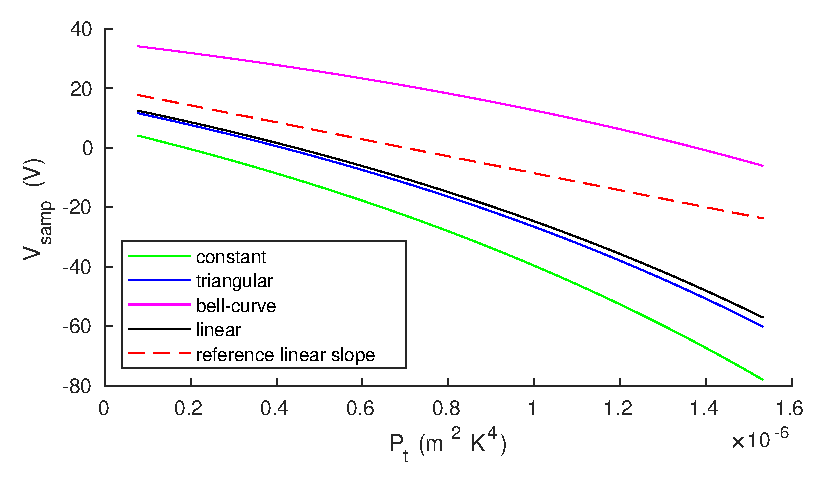
\includegraphics[scale=0.9]{gfx/out_vs_inrad.eps}
  \caption{Power spectrum of output signal for different frame-rates}
  \label{fig:out_vs_inrad}
  \end{center}
\end{figure}

\subsection{Spectrum of the output noise depending on spectrum of input noise}
The noise of the voltage is suspected to contain a component with a
$1/f$ spectrum, so called Flicker noise. It is therefore interesting
to investigate the effect of replacing the noise term in
Equation~\eqref{eq:heat_balance_equation_noise_discr} with a term of $1/f$
spectrum. For a detailed explanation of how such a noise term is
generated, see Section~\ref{sec:flicker-noise}. The power spectrum
of the output noise with $1/f$ noise as input is seen in
Figure~\ref{fig:power_spectrum_pink}.
%\begin{figure}[H]
%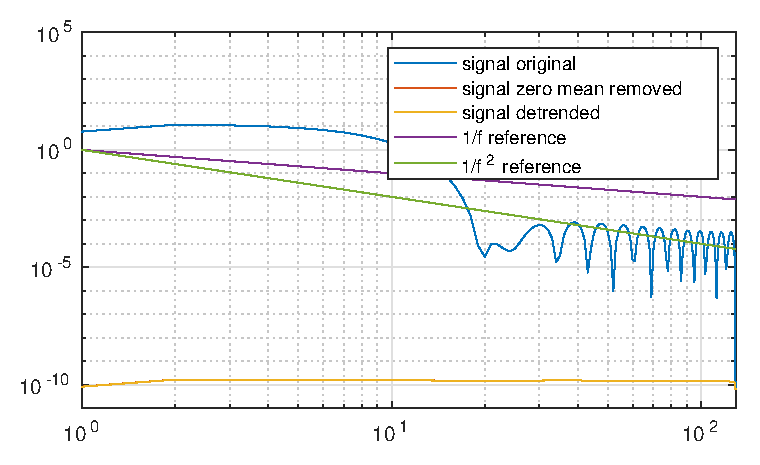
\includegraphics[scale=0.9]{gfx/spectrum_white_noise.eps}
%\caption{Power spectrum with white noise in the input. White noise in the input gives white noise in the output. \gm{Give better explanation in the caption} }
%\label{fig:power_spectrum_white}
%\end{figure}

\begin{figure}[H]
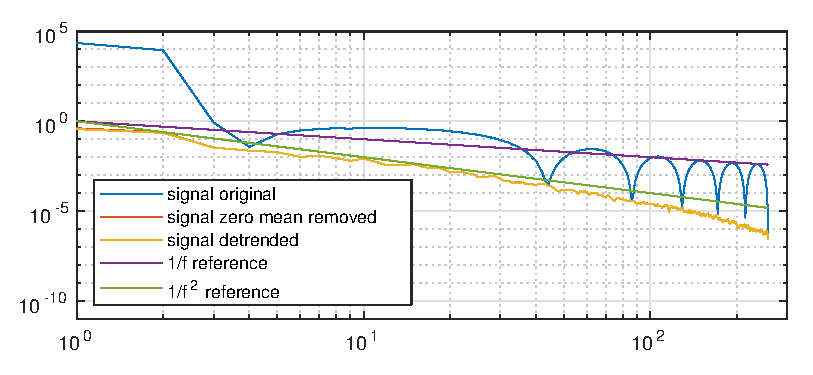
\includegraphics[scale=0.9]{gfx/spectrum_pink_noise.eps}
\caption{Power spectrum with $1/f$ noise in the input.}
\label{fig:power_spectrum_pink}
\end{figure}


%%% Local Variables:
%%% mode: latex
%%% TeX-master: "main"
%%% TeX-PDF-mode: 1
%%% TeX-PDF-via-dvips-ps2pdf: 1
%%% End:
